\addcontentsline{toc}{chapter}{Appendix 8}
\chapter{Vibrations}

\begin{comment}
"Vibration is not just a rocket issue, though. All electronic hardware is tested for its ability to handle shock and vibration. An MP3 player, for example, has to be tested for its ability to handle the vibrations from someone walking or jogging while holding it, placing it on a counter top, or accidentally dropping it on the floor. However, compared to the workout that Ares I-X’s avionics receive, your MP3 player has got it easy. Imagine shaking that MP3 player inside an automatic paint can shaker for two minutes while continuing to play your favourite tunes. That’s kind of what the electronics of the I-X are up against."
\end{comment}

\emph{"Imagine shaking that MP3 player inside an automatic paint can shaker for two minutes while continuing to play your favourite tunes. That's kind of what the electronics are up against."} \cite{MITRocketVibrations}

As discussed before, dynamics can affect the \ac{GNSS} receiver in two fundamental ways. Low frequency dynamics (\ac{QSL}) result in the receiver accelerating, and the nominal carrier frequency changing due to the doppler shift. 

Dynamics can also affect the receiver by placing mechanical loads upon the quartz crystal used as a frequency reference in the receiver. From the receiver's perspective, a change in the carrier frequency is indistinguishable from a change in the local oscillator frequency generated by the quartz crystal\cite{Kaplan}. 

\subsection{Crystals}
Understanding the impact of vibrations on the crystal is vital for understanding the performance that can be expected from the receiver during ascent \& re-entry. While the receivers ability to deal with dynamics can be assessed readily in the laboratory using a GPS simulator, assessing the impact of vibrations on the receiver is somewhat more complex.

While all mechanical stresses on the crystal cause changes in the frequency produced, for analysis purposes, they are typically grouped in into two categories, namely acceleration stresses, and vibration stresses. 

\begin{comment}
http://www.vectron.com/products/g_sensitivity/Vig-tutorial%20on%20g-sensitivity.pdf
\end{comment}

The  Kea receiver uses the Abracon ASVTX-12 \ac{TCXO}\cite{ASTX12Datasheet}, while the flight model Biarri uses the Vectron  VT-803 TCXO\cite{VT803Datasheet}. While information on g sensitivity is not published for either of these \ac{TCXO}, 
Kaplan suggests that a typical value for g sensitivity is $1 ppb/g$ \cite{Kaplan}.

Additionally, much can be discovered from examining the specification of similar models. The TX-705 oscillator is specifically designed for applications where superior g-sensitivity is required. From the data sheet, we can observe that the g sensitivity of the crystal is consistently less than at $0.1ppb/g$ in the range from 20Hz to 2000Hz \cite{TX705Datasheet}. It is reasonable to expect that the performance of the VT-803 and the ASVTX-12 will be somewhat inferior to the TX-705, however the specification provide guidance on the order of magnitude of sensitivity that can be expected.

\subsection{Mitigation}
There are 4 main strategies for mitigation.

\begin{itemize}
\item{Part specification}
\item{Orientation}
\item{Mechanical isolation}
\item{Electrical compensation}
\end{itemize}

\subsubsection{Part specification}
Correctly specifying a receiver with a low g-sensitivity is an effectiv method of reducing the effects of vibration on the reciever. With the current \ac{XO} used on the \ac{NAMURU} board, there is a degree of uncertinty regarding the effect of vibration, because the g-sensitivity is not specified. This is somewhat troublesome, given that it is possible that the sensitivity of different crystals from different batches may differ. Hence a reciever may fail in the field due to vibrations, while a nominally identicall reciever used for development and testing may operate satisfactraly. By chosing parts which meets a minimal standard for g-sensitivity, increased confidence in the performance of the reciever can be gained, at the cost of increased financial outlay. 

\subsubsection{Orientation}
Quartz crystals are anisotropic in nature, so it is not unexpected that the frequency shift is a function of the direction of acceleration. For a typical crystal which is cut for use in g-sensitive applications, there is approximately a two fold difference between the sensitivity between the most and least sensitive axis \cite{CrystalVibration}. Hence judicious orientation of the crystal or receiver can have a significant impact on performance. In the case of liquid fueled rockets, one insidious form of vibration is POGO, a type of self excited combustion osciallation in liquid fuled rocket engines\cite{Pogo}. 

While this type of vibration has largely been eliminated through careful engineering design, in a system which may be su


\subsubsection{Mechanical isolation}
By mounting the PCB which the \ac{NAMURU} receiver is mounted on in an approiate matter, vibratoins can be mechanically suppressed. Judicious application of mechanical dampers where the board is mounted can be effective in preventing the transmission of high frequency vibrations to the board. 

\subsubsection{Electrical compensation}
Electrical compensation uses an acceleromter to bias the output from the crystal depending on the acceleration being experiened. This method is an analog for the control scheme used in an \ac{TCXO} \cite{CrystalVibration}. 


\subsection{Determining g-sensitivity}
There are three main methods for determining the the g-sensitivity of the receiver.

\begin{itemize}
\item{Manufacturers data sheet}
\item{2g Tip over test}
\item{Vibration testing}
\end{itemize}

Manufacturers datasheets are a preferred solution, however the g-sensitivity may not be provided, especially if the \ac{TCXO} is not designed with g-sensitivity in mind. Additionally,  the g-sensitivity of a \ac{TCXO} may be commercial in confidence, with manufacturer unwilling to share the performance of their crystal, especially for a university who is not going to mass produce a design using that part. 

One simple method of determining the g-sensitivity of the crystal is the 2g tip over test. The test is conceptually simple, and is carried out in the following manner:

\begin{enumerate}
\item{Measure the frequency output of the crystal in one orientation}
\item{Rotate the crystal 180 \degree about an axis}
\item{Measure the frequency output again}
\end{enumerate}

 The g-sensitivity can be found as:

\begin{equation}
\frac{f_1-f_2}{2 f_1}\text{ ppb/g}
\end{equation}

A final method is to place the crystal on a vibrating table. 

\begin{comment}
In recent years significant progress has been made in
crystal resonator design to effect a substantial reduction in
g-sensitivity values [1]. With such reduced levels of
acceleration sensitivity, the need has arisen for a
measurement system with appropriately higher resolution.
The most obvious method for determination of g-sensitivity
for a stable ovenized oscillator is the '2g tip over
test', where the whole oscillator is simply inverted, resulting
in an incremental 2g change in the internal forces applied to
the resonator [2]. However, since the changes are in the
order of 1.10-9 per g, the oscillator temperature must be prestabilized,
and this can be a long process. With this method,
care must also be taken to avoid convectional temperature
effects in the oven cavity, which can cause misleading
results.
In this work, for g-sensitivity measurement, the method
that has been implemented is based on the imposition of an
essentially sinusoidal low frequency vibration field on the
resonator by placing the device on a vibration table, and
then observing the modulation effects on the resonator
frequency.
The method is applicable to any repetitive stimulus to
which the frequency of the resonator exhibits sensitivity.
Such stimuli could include pressure, electromagnetic
radiation effects, magnetic fields, neutron radiation, and so
on.
\end{comment}

%\cite{2GTipover}


\subsection{Acceleration stresses}

\begin{equation}
\Delta f_g = 360 S_g f_L G(t) (\degree/s)
\end{equation}
%\cite{Kaplan}

\begin{align*}
S_g &= \text{g-sensitivity of the oscillator (}\Delta \text{f/f per g)}\\
f_L &= \text{1,575.42 MHz for L1} \\
G(t) &= \text{acceleration stress in g as a function of time}
\end{align*}


\begin{table}[!htb]
\centering
\begin{tabular}{|l|l|l|}
\hline
\rowcolor[HTML]{C0C0C0} 
Environment                 & Acceleration (g) & $\Delta f$ (Hz) \\ \hline
Buildings                  & 0.02        &    0.03\\ \hline
\rowcolor[HTML]{EFEFEF} 
Ship (Calm Seas)           & 0.02-0.1    &  0.03-0.2     \\ \hline
Ship (Rough Seas)          & 0.8    &     1          \\ \hline
\rowcolor[HTML]{EFEFEF} 
Train                      & 0.1-1        & 0.2-2              \\ \hline
Jet aircraft               & 0.1-2        & 0.2-3              \\ \hline
\rowcolor[HTML]{EFEFEF} 
Armoured Personnel Carrier & 0.5-3         &  0.8-5             \\ \hline
Propeller aircraft         & 0.3-5         & 0.5-8             \\ \hline
\rowcolor[HTML]{EFEFEF} 
Helicopter                 & 0.3-7         & 0.5-11              \\ \hline
Missile (Boost phase)      & 15          &  24             \\ \hline
\end{tabular}
\caption{\cite{CrystalVibration}}
\label{VibrationLevelsTable}
\end{table}

\subsection{Vibration stresses}
Equation 5.8
\begin{equation}
\sigma_v = \frac{360f_L}{2\pi}\sqrt{\int_{f_{min}}^{f_{max}} S^2_v(f_m) \frac{P(f_m)}{f^2_m} df_m}\text{ (degrees)}
\end{equation}
%\cite{Kaplan}

\begin{equation}
\sigma_v = \frac{\lambda_L}{2\pi}\sqrt{\int_{f_{min}}^{f_{max}} S^2_v(f_m) \frac{P(f_m)}{f^2_m} df_m}\text{ (meters)}
\end{equation}
%\cite{Kaplan}

\begin{align*}
f_L &= \text{L-band input frequency in Hz} \\
S_v(f_m) &= \text{oscillator vibration sensitivity of } \Delta f/f_L \text{ per g as a function of } f_m \\
f_m &= \text{random vibration modulation frequency in Hz} \\
P(f_m) &= \text{power curve of the random vibration in }g^2/Hz \text{ as a function of } f_m \\
g &= \text{acceleration due to gravity} \approx 9.8 m/s^2
\end{align*}



\begin{itemize}
\item{Thrust oscillations\cite{NASAVibrations}}
\item{Noise (pressure waves) due to the motor or
engine (liftoff, transonic, max dynamic pressure)\cite{NASAVibrations}}
\item{Pyroshocks (explosive bolts and such)\cite{HarveyMudd}}
\item{Winds\cite{HarveyMudd}}
\item{Turbulence\cite{HarveyMudd}}
\item{Turbomachinery (liquid propellant engines)\cite{HarveyMudd}}
\end{itemize}

\begin{figure}[!htb] 
    \centering
    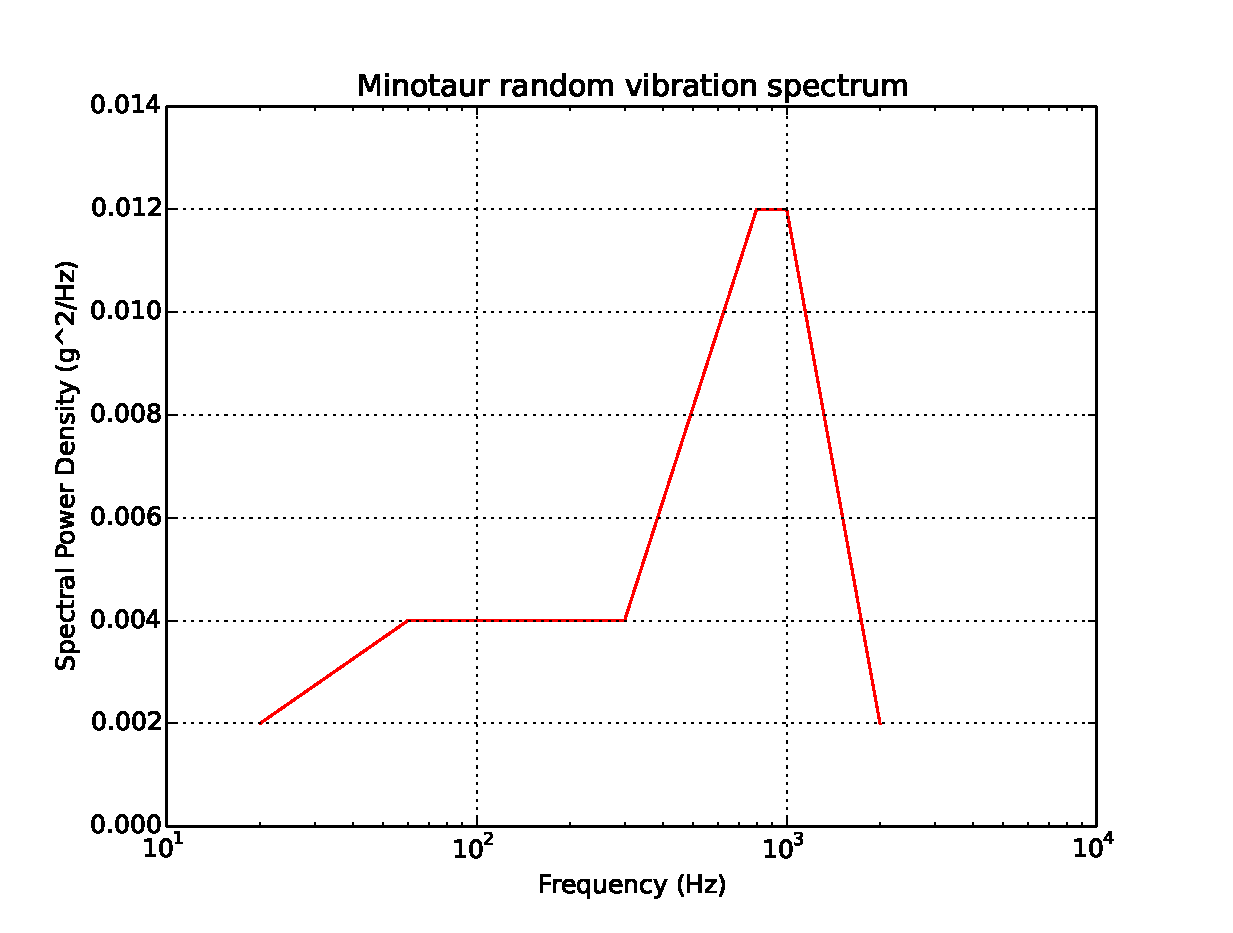
\includegraphics[width=1\textwidth]{Vibrations/Minotaur.eps} 
    \caption{Integral is 14.48 $g^2$, phase error is $1.2\degree$, for a crystal with a g-sensitivity of  1ppb/g.}
    \label{fig:MinotaurVibrations}
\end{figure}


\begin{figure}[!htb] 
    \centering
    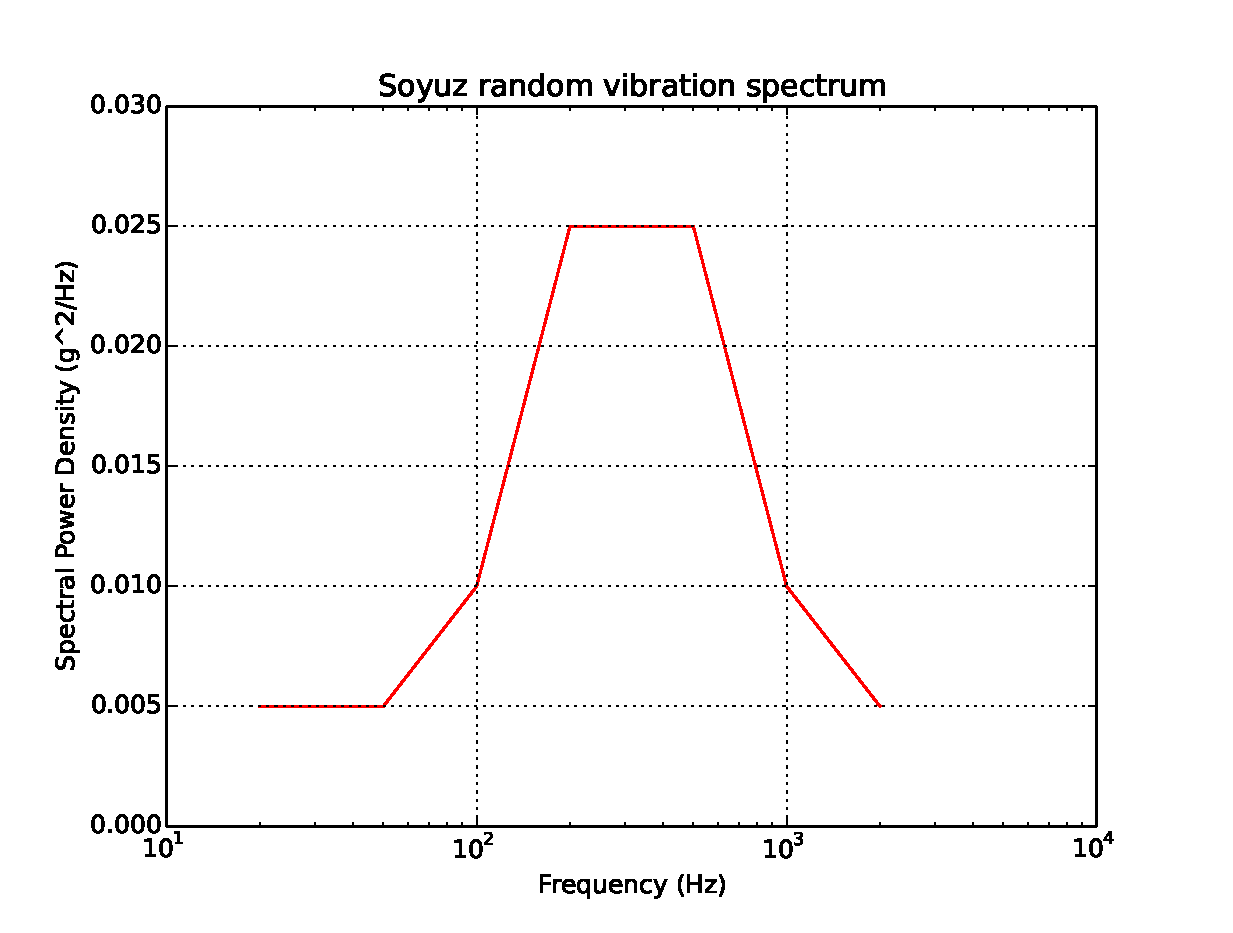
\includegraphics[width=1\textwidth]{Vibrations/Soyuz.eps} 
    \caption{Integral is 26.025 $g^2$, phase error is $1.8\degree$, for a crystal with a g-sensitivity of  1ppb/g.}
    \label{fig:SoyuzVibrations}
\end{figure}

\begin{figure}[!htb] 
    \centering
    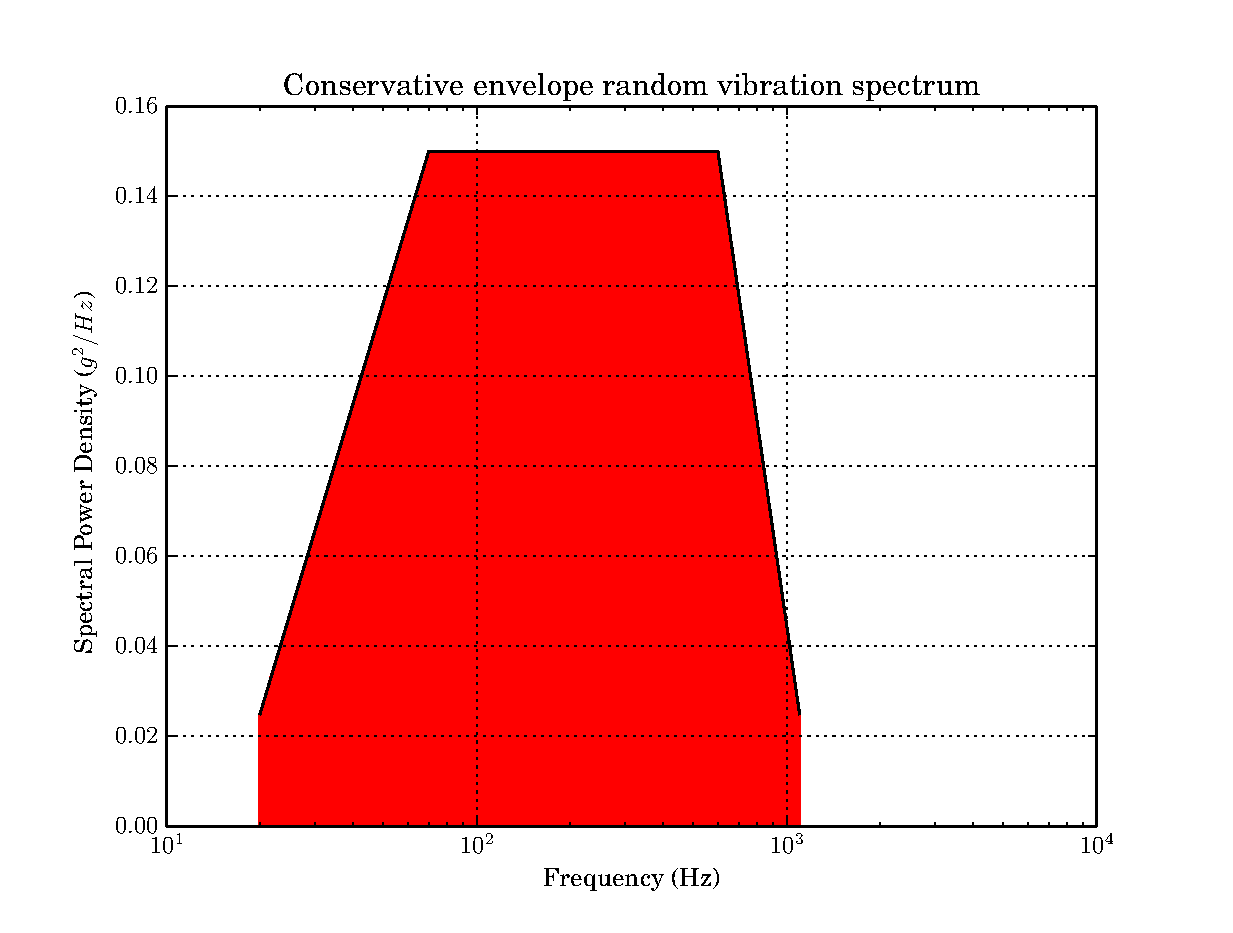
\includegraphics[width=1\textwidth]{Vibrations/Envelope.eps} 
    \caption{A conservative vibration spectrum envelope, from \cite{VibrationHandout}. Phase error is $5.9\degree$, for a crystal with a g-sensitivity of  1ppb/g.}
    \label{fig:ConservativeVibrations}
\end{figure}



\subsection{Shock stresses}
Space Exploration Technologies Corp  specifies four main shock events
\cite{Falcon9}: 
\begin{itemize}
\item{Vehicle hold-down release at lift-off} 
\item{2nd stage separation}
\item{Fairing separation}
\item{Payload release and separation}
\end{itemize}

\subsection{Acoustic stresses}
During launch, the \ac{LV} experiences a challenging acoustic environment. Noise from the rocket motors has a tendency to deflect from the ground and surrounding structures, impacting the launch vehicle. If acoustic pressure waves, mechanically couple with the \ac{PCB} which \ac{NAMURU}, then this may lead to additional vibrations which may further degrade performance. Fortunately, the most acoustically challenging time is at launch, which is when for a successful launch, dynamics are at their lowest. 

Conversely, in the event of a launch failure, the launch abort system may be used to extradite the crew capsule away from the \ac{LV}. In this scenario, the receiver will experience significant dynamics, while also being exposed to significant acoustic stresses. In the case of the \ac{LV} detonating, then an intense shock-wave is likely to impact the receiver. While this scenario is not unprecedented in the history of spaceflight, positioning provided by an \ac{IMU} is likely to be satisfactory in this case.


\subsection{Antenna phase-centre displacement}
One effect that is often overlooked, is that the antenna is physically displaced. Because the LOS distance is between the satellite antenna phase centre and the receiver phase centre, the physical movement of the antenna can have a detrimental effect on the receiver. From an analytical point of view, moving the antenna phase centre results in a change in detected frequency,  ASK EAMONN.

While no empirical formula for analysis of this issue were uncovered during the literature review, this issue represents an opportunity for further analysis. During testing, this effect can be accounted for by performing the vibration test in an anechoic chamber, and transmitting a signal wireless to a vibrating receiver/antenna assembly. 


Equation 5.8
\begin{equation}
\sigma_v = \frac{360f_L}{2\pi}\sqrt{\int_{f_{min}}^{f_{max}} S^2_v(f_m) \frac{P(f_m)}{f^2_m} df_m}\text{ (degrees)}
\end{equation}
%\cite{Kaplan} \cite{Jwo}

Where:
\begin{align*}
f_L &= \text{L-band input frequency in Hz} \\
S_v(f_m) &= \text{oscillator vibration sensitivity of } \Delta f/f_L \text{ per g as a function of } f_m \\
f_m &= \text{random vibration modulation frequency in Hz} \\
P(f_m) &= \text{power curve of the random vibration in } g^2/Hz \text{ as a function of } f_m \\
g &= \text{ acceleration due to gravity } \approx 9.8 m/s^2\\
\end{align*}


Equation 5.16
Talk about the 2G tip-over test
\begin{equation}
\Delta f_g = 360 S_g f_L G(t) (\degree/s)
\end{equation}
%\cite{Kaplan}

Where:
\begin{align*}
S_g &= \text{g-sensitivity of the oscillator } (\Delta \text{ f/f per g)}\\ 
f_L &= \text{L-band input frequency (Hz)}\\
&= \text{1,575.42 MHz for L1}\\
G(t) &= \text{acceleration stress in g as a function of time}
\end{align*}


